\documentclass[11pt,a4paper]{article}
\usepackage[UTF8]{ctex}
\usepackage{graphicx}
\graphicspath{{report/figures/}{figures/}}
\usepackage{amsmath,amssymb}
\usepackage{booktabs}
\usepackage{array}
\usepackage{adjustbox}
\usepackage{float}
\usepackage{hyperref}
\usepackage{listings}
\usepackage{xcolor}
\usepackage[a4paper,margin=2.5cm]{geometry}
\usepackage{enumitem}
\usepackage{url}
\usepackage[numbers]{natbib}
\usepackage{fancyhdr}
\setlength{\headheight}{14pt}
\pagestyle{fancy}
\fancyhf{}
\fancyhead[C]{VIB PhaseLab 实验报告}
\fancyfoot[C]{\thepage}

\lstset{
    language=Python,
    basicstyle=\footnotesize\ttfamily,
    breaklines=true,
    frame=single,
    keywordstyle=\color{blue},
    commentstyle=\color{teal},
    stringstyle=\color{red!70!black}
}

\title{\bf 信息论课程报告\\[0.5em]
\Large VIB PhaseLab：基于变分信息瓶颈的表示压缩、鲁棒性相变与诊断系统}
\author{姓名：\underline{~~~~~~~~~叶盛豪~~~~~~~~~} \quad 学号：\underline{~~~~~PB24000227~~~~~~}}
\date{2026 年 6 月 8 日}

\begin{document}
\maketitle

\begin{abstract}
信息瓶颈理论将表示学习描述为“保留任务相关信息、压缩输入冗余信息”的优化问题。变分信息瓶颈（Variational Information Bottleneck, VIB）进一步将这一思想转化为可训练的神经网络目标，通过在交叉熵损失之外加入 KL 正则项，使模型学习随机潜变量表示，并用瓶颈系数 $\beta$ 控制表示压缩强度。

本报告围绕“表示压缩何时提升泛化与鲁棒性，何时破坏任务信息”这一问题，完成了 VIB-CNN 的复现、扩展实验和交互式诊断系统构建。基础复现实验比较普通 CNN 与 VIB-CNN 在 MNIST 和 Fashion-MNIST 上的 clean accuracy、Gaussian noise 鲁棒性、KL proxy 与 latent PCA 结构。进一步地，本人设计并实现了 VIB PhaseLab：在 MNIST、Fashion-MNIST 和 CIFAR-10 三个数据集上，系统扫描 CNN baseline 与 VIB-CNN 的 12 个 $\beta$ 配置，并在 Gaussian、salt-and-pepper、blur、contrast 四类 corruption 与五个 severity 上进行鲁棒性评测，共得到 39 个真实实验配置和 780 条 corruption robustness 评测记录。

实验结果表明，$\beta$ 对表示压缩具有显著控制作用，但压缩并不自动等价于鲁棒性提升。MNIST 上，$\beta=0.03$ 的 VIB-CNN 达到最高 clean accuracy 99.39\%，并在 salt-and-pepper corruption 上取得最佳 robustness AUC 0.9474；Fashion-MNIST 上，$\beta=0.03$ 取得最高 clean accuracy 92.29\%，但 Gaussian 与 salt-and-pepper 的最佳鲁棒性仍来自 CNN baseline；CIFAR-10 上，$\beta=0.003$ 取得最高 clean accuracy 70.41\%，而不同 corruption 的最优模型分散在 CNN baseline 与不同 $\beta$ 的 VIB-CNN 之间。上述现象说明，VIB 更适合被视为一种可诊断、可调节的压缩正则化机制，而不是通用鲁棒性保证。

\noindent\textbf{关键词}：信息瓶颈；变分信息瓶颈；表示压缩；鲁棒泛化；相变分析；VIB PhaseLab
\end{abstract}

\section{引言}

深度神经网络的中间表示通常同时包含任务相关信息和输入细节信息。对于图像分类任务而言，模型既需要保留类别判别所需的结构信息，又可能无意中记住背景、纹理、噪声和训练集偶然模式。信息论提供了一种分析这一现象的视角：如果将输入记为 $X$，标签记为 $Y$，中间表示记为 $Z$，那么好的表示应当在保留关于 $Y$ 的信息的同时，尽可能压缩关于 $X$ 的冗余信息。

信息瓶颈目标可写为：
\begin{equation}
\max I(Z;Y)-\beta I(Z;X),
\end{equation}
其中 $I(Z;Y)$ 衡量表示中的任务相关信息，$I(Z;X)$ 衡量表示中保留的输入信息，$\beta$ 控制压缩强度。直观上，较小的 $\beta$ 允许模型保留更多输入细节，较大的 $\beta$ 则强迫模型学习更紧凑的表示。然而，在实际神经网络中，压缩与泛化之间的关系并不总是单调的：适度压缩可能去除噪声和冗余，提高泛化；过度压缩则可能抹去标签相关信息，导致欠拟合。

本文关注的问题是：\textbf{VIB 的压缩何时是 useful compression，何时变成 destructive over-compression？} 为回答这一问题，本项目不只复现 VIB-CNN，而是构建了一个完整的 PhaseLab 实验系统：
\begin{itemize}[leftmargin=2em]
    \item 从信息瓶颈目标出发，实现普通 CNN 与 VIB-CNN 的可复现实验管线；
    \item 在 MNIST、Fashion-MNIST 和 CIFAR-10 上扫描多组 $\beta$，比较 clean accuracy、KL proxy 和多类型 corruption 鲁棒性；
    \item 设计 robustness AUC、compression benefit index、KL collapse score 与 phase label，刻画表示压缩的阶段变化；
    \item 计算 latent geometry 与 latent drift，分析压缩对表示空间结构的影响；
    \item 构建 FastAPI + React/Vite 的中文 Dashboard，使实验结果可以交互式展示和复核。
\end{itemize}

\section{相关工作}

\textbf{信息瓶颈理论。} 信息瓶颈理论最早将表示学习表述为压缩输入信息并保留任务相关信息的优化问题。对于监督学习任务，理想表示 $Z$ 应当舍弃与标签无关的输入扰动，同时保留足够的类别判别信息。

\textbf{变分信息瓶颈。} Alemi 等人提出的 Variational Information Bottleneck 将 IB 目标转化为可优化的变分形式。其核心做法是令编码器输出潜变量分布 $q_\phi(z|x)$，并用先验 $p(z)$ 约束潜变量，使 $KL(q_\phi(z|x)||p(z))$ 成为 $I(X;Z)$ 的可计算上界。

\textbf{鲁棒泛化与输入扰动。} 模型在 clean test set 上表现良好并不意味着它对输入扰动稳健。Gaussian noise、salt-and-pepper noise、blur 和 contrast corruption 分别破坏像素值、局部像素、空间细节和整体强度分布。多 corruption 评测比单一噪声更能揭示表示的鲁棒性结构。

\section{方法}

\subsection{CNN baseline 与 VIB-CNN}

普通 CNN baseline 使用卷积编码器将输入图像映射为 latent representation，再通过线性分类器输出类别 logits。训练目标为标准交叉熵：
\begin{equation}
\mathcal{L}_{\text{CNN}}=CE(\hat{y},y).
\end{equation}

VIB-CNN 使用与 CNN baseline 相近的卷积骨干，但编码器输出均值 $\mu(x)$ 与对数方差 $\log\sigma^2(x)$，定义潜变量分布：
\begin{equation}
q_\phi(z|x)=\mathcal{N}(\mu(x),\operatorname{diag}(\sigma^2(x))).
\end{equation}
训练时使用重参数化技巧：
\begin{equation}
z=\mu(x)+\sigma(x)\odot\epsilon,\quad \epsilon\sim\mathcal{N}(0,I).
\end{equation}
损失函数为：
\begin{equation}
\mathcal{L}_{\text{VIB}}=CE(\hat{y},y)+\beta KL(q_\phi(z|x)||p(z)),
\end{equation}
其中 $p(z)=\mathcal{N}(0,I)$。本文报告中的 average KL 是测试集上的平均 KL proxy，用作 $I(X;Z)$ 的变分上界近似，而不是精确互信息估计。

\subsection{Phase indicators}

PhaseLab 使用四类指标刻画压缩阶段。对于 corruption $c$，robustness AUC 定义为不同 severity 下 accuracy 的平均值：
\begin{equation}
AUC_c=\frac{1}{|S|}\sum_{s\in S}Acc(c,s).
\end{equation}
归一化鲁棒性 AUC 为：
\begin{equation}
\widetilde{AUC}_c=\frac{AUC_c}{Acc_{clean}}.
\end{equation}
Compression Benefit Index 使用同一数据集 CNN baseline 作为参考：
\begin{equation}
CBI_c=\widetilde{AUC}_{c,\text{VIB}}-\widetilde{AUC}_{c,\text{CNN}}.
\end{equation}
KL collapse score 使用同一数据集 VIB $\beta=0$ 的 KL 作为参考：
\begin{equation}
\text{KL-collapse}=\frac{KL_\beta}{KL_{\beta=0}}.
\end{equation}

系统根据 clean accuracy drop、CBI 和 KL collapse score 给每个配置赋予诊断标签：压缩不足、有效压缩、鲁棒特化、过度压缩或不稳定。该标签是实验诊断工具，不是理论定理。

\section{实验设置}

\subsection{硬件与软件环境}

\begin{table}[H]
\centering
\caption{实验硬件与软件环境}
\begin{tabular}{ll}
\toprule
配置项 & 详情 \\
\midrule
服务器 & Tang-2-Wu \\
GPU & NVIDIA A40 48GB（使用单卡） \\
Python 环境 & /data/wujcan/yesh/miniconda3/envs/tn\_env \\
PyTorch / Torchvision & 2.7.1+cu126 / 0.22.1+cu126 \\
运行目录 & /NAS/yesh/vib-robustness-lab \\
关键环境变量 & VIB\_DISABLE\_CUDNN=1, PYTHONPATH=src \\
前端 / 后端 & React + TypeScript + Vite / FastAPI \\
\bottomrule
\end{tabular}
\end{table}

\subsection{实验矩阵}

\begin{table}[H]
\centering
\caption{PhaseLab 实验矩阵}
\begin{tabular}{ll}
\toprule
维度 & 配置 \\
\midrule
数据集 & MNIST, Fashion-MNIST, CIFAR-10 \\
模型 & CNN baseline, VIB-CNN \\
$\beta$ grid & 0, 1e-5, 3e-5, 1e-4, 3e-4, 1e-3, 3e-3, 1e-2, 3e-2, 1e-1, 3e-1, 1 \\
Corruption & Gaussian, salt-and-pepper, blur, contrast \\
Severity & 0.0, 0.1, 0.2, 0.3, 0.4 \\
Epoch & 10 \\
Latent dimension & 32 \\
\bottomrule
\end{tabular}
\end{table}

每个数据集包含 1 个 CNN baseline 和 12 个 VIB-CNN 配置，因此总计 39 个实验配置。每个配置在 4 类 corruption 和 5 个 severity 上评测，因此总计 780 条 robustness 记录。

\section{实验结果}

\subsection{基础 VIB 复现实验}

在 MNIST 上，普通 CNN baseline 的 clean accuracy 为 98.81\%，train-test gap 为 0.76\%。VIB-CNN 在 $\beta=0.1$ 时取得最高 clean accuracy 99.38\%，比 CNN baseline 高 0.57 个百分点；此时 KL proxy 为 4.7760，明显低于 $\beta=0$ 时的 872.7278。当 $\beta=1$ 时，MNIST clean accuracy 降至 64.10\%，KL proxy 降至 0.0433，体现了过度压缩现象。

在 Fashion-MNIST 上，CNN baseline 的 clean accuracy 为 90.50\%，train-test gap 为 2.82\%。VIB-CNN 在 $\beta=0.01$ 时取得最高 clean accuracy 92.17\%，比 CNN baseline 高 1.67 个百分点；此时 KL proxy 为 11.5234，相比 $\beta=0$ 的 316.1828 大幅下降。当 $\beta=1$ 时，Fashion-MNIST clean accuracy 降至 60.14\%，KL proxy 降至 0.0210。

\subsection{PhaseLab clean accuracy 总览}

\begin{table}[H]
\centering
\caption{各数据集 clean accuracy 最佳配置}
\begin{adjustbox}{max width=\textwidth}
\begin{tabular}{llllrrr}
\toprule
数据集 & 最佳实验 & 模型 & $\beta$ & Clean Acc. & Avg. KL & KL collapse \\
\midrule
MNIST & mnist\_vib\_beta\_0\_03 & VIB-CNN & 0.03 & 99.39\% & 7.0490 & 0.0081 \\
Fashion-MNIST & fashion\_mnist\_vib\_beta\_0\_03 & VIB-CNN & 0.03 & 92.29\% & 7.5336 & 0.0238 \\
CIFAR-10 & cifar10\_vib\_beta\_0\_003 & VIB-CNN & 0.003 & 70.41\% & 25.8218 & 0.1398 \\
\bottomrule
\end{tabular}
\end{adjustbox}
\end{table}

三个数据集的最佳 clean accuracy 均由 VIB-CNN 取得，说明适当 $\beta$ 的信息瓶颈确实能发挥正则化作用。不过，最佳 clean 配置并不一定是所有 corruption 下最鲁棒的配置。

\begin{figure}[H]
\centering
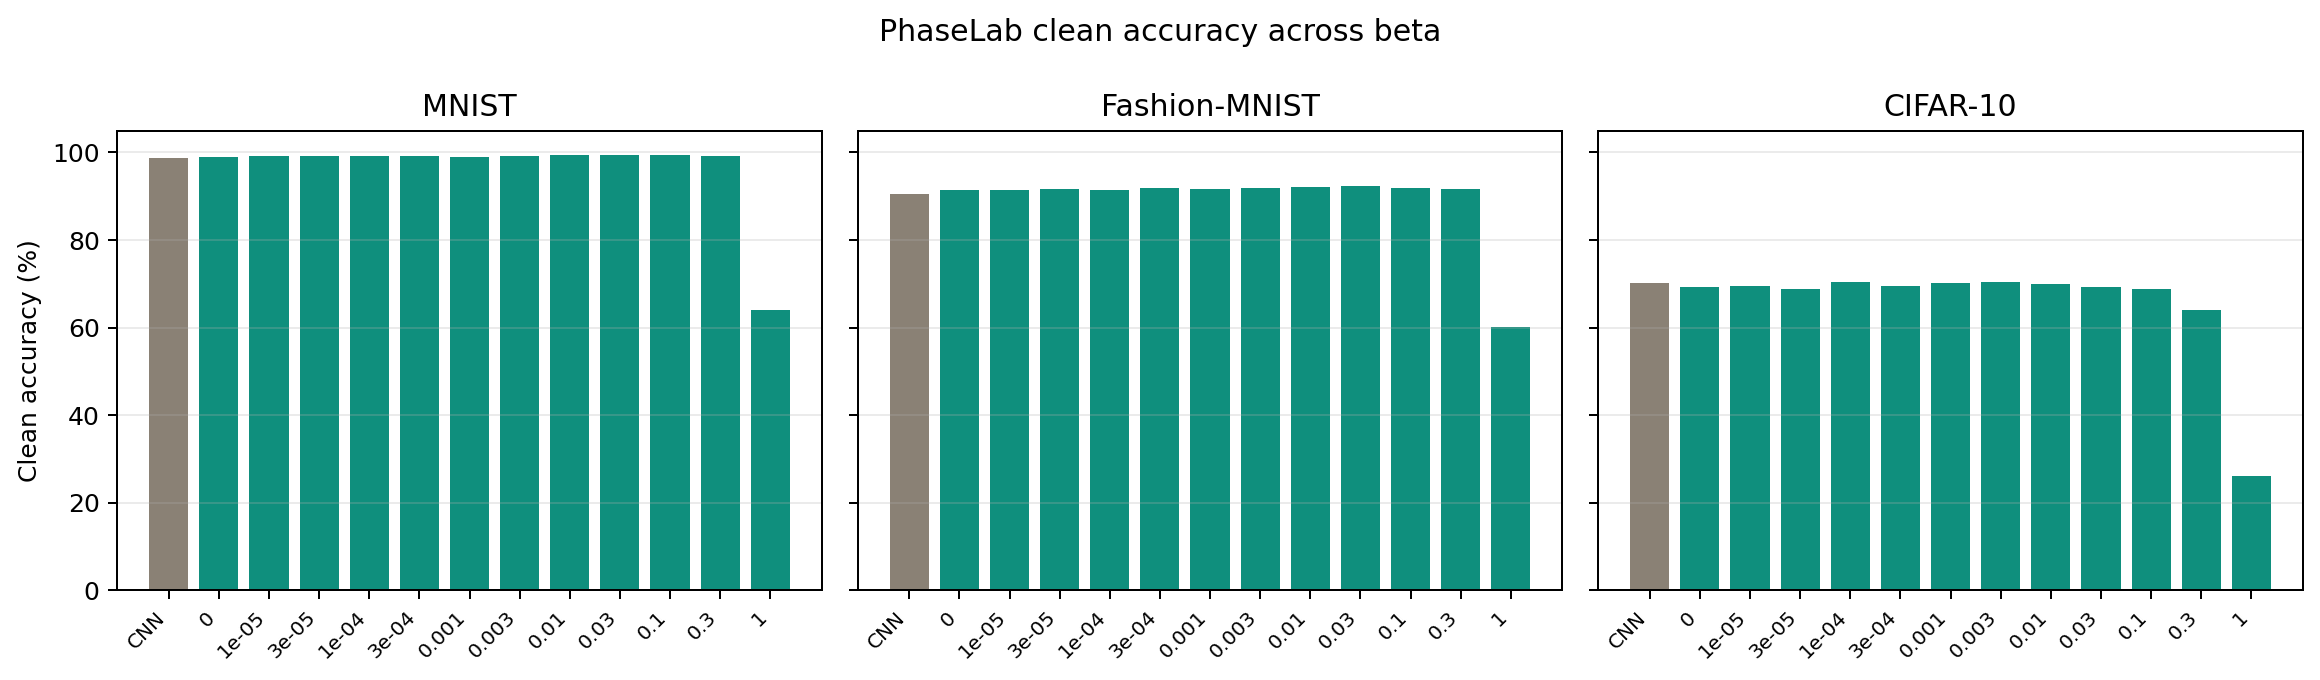
\includegraphics[width=0.95\textwidth]{phaselab_clean_accuracy.png}
\caption{PhaseLab 中 CNN baseline 与不同 $\beta$ 的 VIB-CNN clean accuracy 对比}
\end{figure}

\begin{figure}[H]
\centering
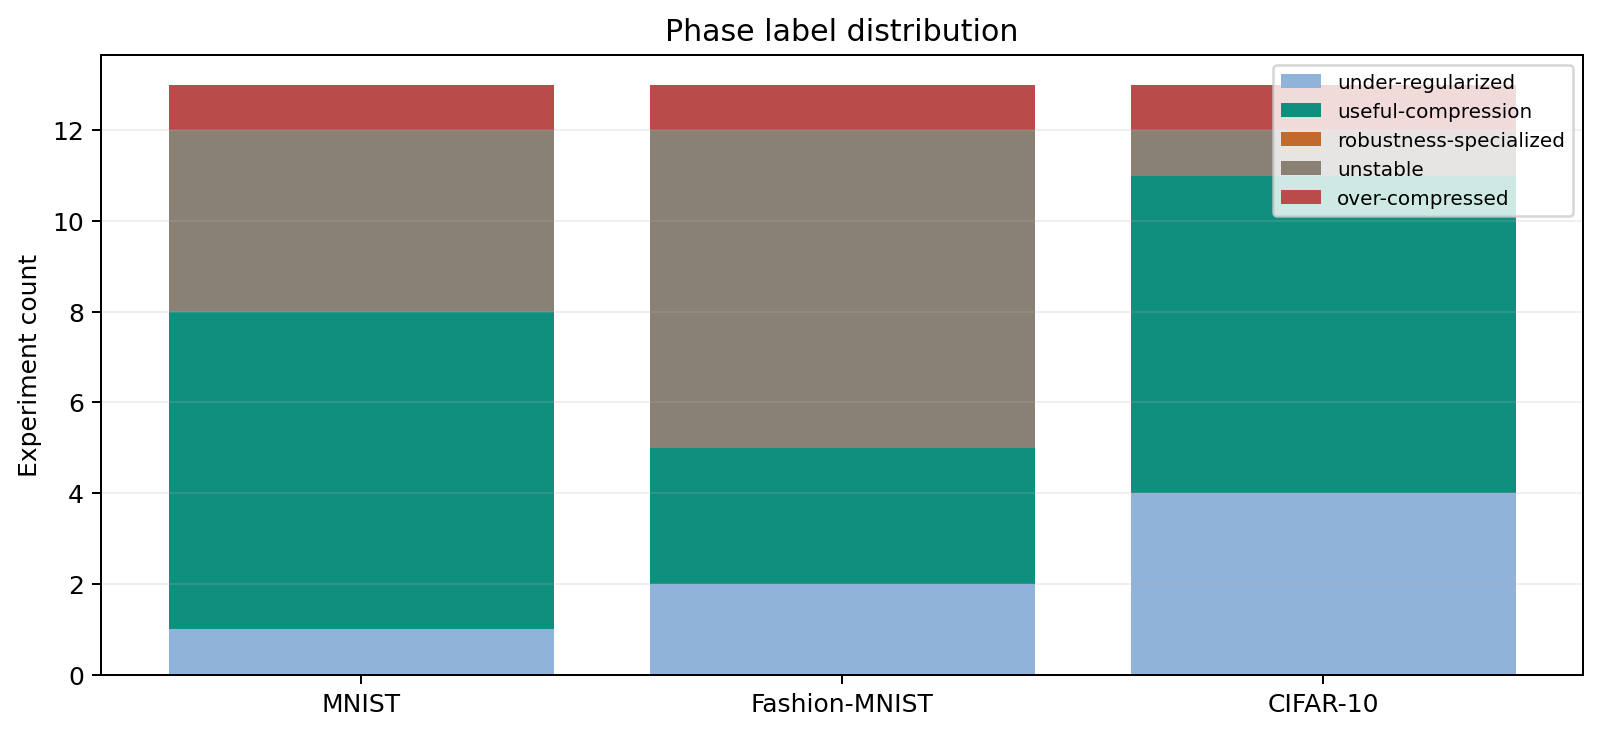
\includegraphics[width=0.82\textwidth]{phaselab_phase_counts.png}
\caption{三个数据集上的 phase label 分布}
\end{figure}

\begin{figure}[H]
\centering
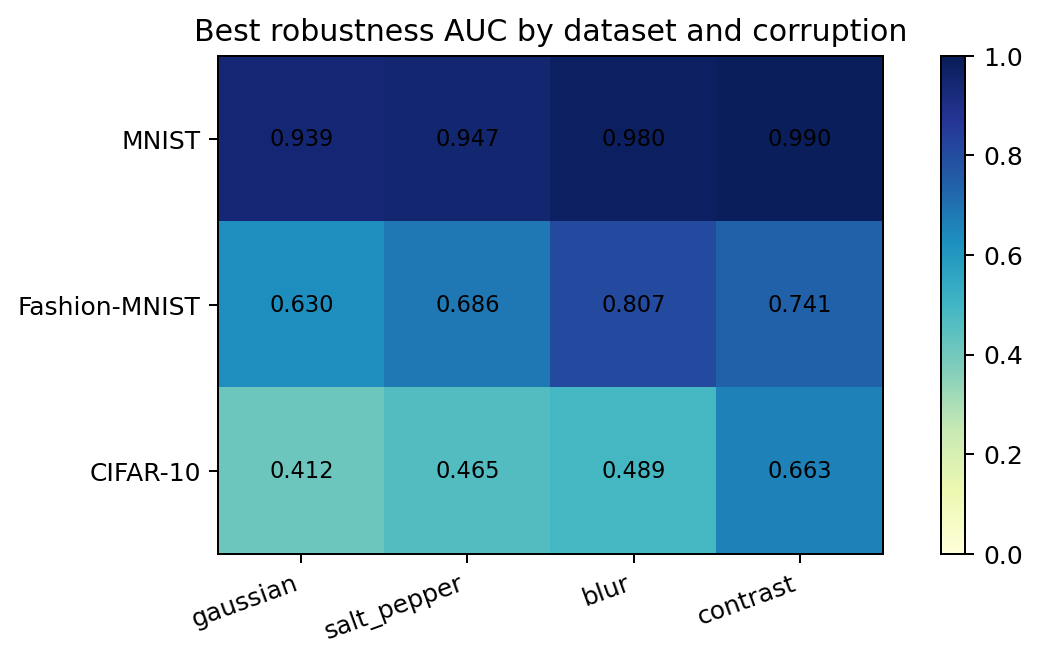
\includegraphics[width=0.82\textwidth]{phaselab_robustness_auc.png}
\caption{各数据集和 corruption 下的最佳 robustness AUC}
\end{figure}

\subsection{MNIST：有效压缩较稳定}

MNIST 的 phase label 分布为：useful-compression 7 个、under-regularized 1 个、unstable 4 个、over-compressed 1 个。MNIST 各 corruption 的最优配置如下：

\begin{table}[H]
\centering
\caption{MNIST 各 corruption 最优 robustness AUC}
\begin{adjustbox}{max width=\textwidth}
\begin{tabular}{llllrr}
\toprule
Corruption & 最优实验 & $\beta$ & AUC & CBI & Clean Acc. \\
\midrule
blur & mnist\_vib\_beta\_0\_0003 & 0.0003 & 0.9799 & 0.0081 & 99.15\% \\
contrast & mnist\_vib\_beta\_3em05 & 0.00003 & 0.9899 & 0.0023 & 99.17\% \\
gaussian & mnist\_vib\_beta\_0 & 0 & 0.9394 & 0.0107 & 98.96\% \\
salt-pepper & mnist\_vib\_beta\_0\_03 & 0.03 & 0.9474 & 0.0025 & 99.39\% \\
\bottomrule
\end{tabular}
\end{adjustbox}
\end{table}

四类 corruption 的最优鲁棒性均由 VIB-CNN 获得，且 CBI 均为正。这说明在 MNIST 这类低复杂度任务中，VIB 压缩较容易去除冗余输入变化，同时保留类别结构。

\subsection{Fashion-MNIST：压缩收益依赖扰动类型}

Fashion-MNIST 的 phase label 分布为：useful-compression 3 个、under-regularized 2 个、unstable 7 个、over-compressed 1 个。最优 robustness AUC 如表所示：

\begin{table}[H]
\centering
\caption{Fashion-MNIST 各 corruption 最优 robustness AUC}
\begin{adjustbox}{max width=\textwidth}
\begin{tabular}{llllrr}
\toprule
Corruption & 最优实验 & $\beta$ & AUC & CBI & Clean Acc. \\
\midrule
blur & fashion\_mnist\_vib\_beta\_1em05 & 0.00001 & 0.8067 & 0.0062 & 91.50\% \\
contrast & fashion\_mnist\_vib\_beta\_0\_003 & 0.003 & 0.7408 & 0.0171 & 91.98\% \\
gaussian & fashion\_mnist\_cnn\_baseline & 0 & 0.6302 & 0.0000 & 90.50\% \\
salt-pepper & fashion\_mnist\_cnn\_baseline & 0 & 0.6859 & 0.0000 & 90.50\% \\
\bottomrule
\end{tabular}
\end{adjustbox}
\end{table}

VIB 在 blur 和 contrast 上取得最优，但 Gaussian 与 salt-and-pepper 的最优结果仍来自 CNN baseline。这说明 VIB 对不同扰动类型的影响并不一致。

\subsection{CIFAR-10：复杂任务上的混合结论}

CIFAR-10 的 phase label 分布为：useful-compression 7 个、under-regularized 4 个、unstable 1 个、over-compressed 1 个。最优 robustness AUC 如表所示：

\begin{table}[H]
\centering
\caption{CIFAR-10 各 corruption 最优 robustness AUC}
\begin{adjustbox}{max width=\textwidth}
\begin{tabular}{llllrr}
\toprule
Corruption & 最优实验 & $\beta$ & AUC & CBI & Clean Acc. \\
\midrule
blur & cifar10\_vib\_beta\_1em05 & 0.00001 & 0.4889 & 0.0384 & 69.59\% \\
contrast & cifar10\_cnn\_baseline & 0 & 0.6625 & 0.0000 & 70.20\% \\
gaussian & cifar10\_cnn\_baseline & 0 & 0.4116 & 0.0000 & 70.20\% \\
salt-pepper & cifar10\_vib\_beta\_0\_01 & 0.01 & 0.4645 & 0.0031 & 70.04\% \\
\bottomrule
\end{tabular}
\end{adjustbox}
\end{table}

CIFAR-10 上，VIB 在 blur 和 salt-and-pepper 上略有优势，但 contrast 和 Gaussian 最优仍是 CNN baseline。这说明在复杂自然图像上，表示压缩的效果受模型容量、数据分布和扰动类型共同制约。

\section{交互式系统实现}

后端位于 `backend/`，使用 FastAPI 只读 artifacts，不执行训练。它提供原始实验索引、单实验详情、PhaseLab 索引、summary 和单实验详情等接口。前端位于 `frontend/`，使用 React、TypeScript、Vite 和 Recharts，包含 Phase overview、phase map、Compression Lens、Diagnosis Lab 和原始 VIB 实验台。

本项目采用 artifact-driven 设计：离线训练生成 JSON artifacts，后端只读服务提供数据，前端负责交互式展示，报告从同一批 artifacts 中归纳结论。这种结构保证了实验结果可复查，并使展示系统不依赖 GPU。

\section{工程实践与验证}

最终验证命令包括：
\begin{lstlisting}[language=bash]
python -m pytest -v
python scripts/validate_phase_artifacts.py artifacts/phase
python scripts/summarize_phase_results.py --artifact-root artifacts/phase --output-dir report/phase_results
python scripts/generate_phaselab_report.py --phase-root artifacts/phase --result-root report/phase_results --output report/phaselab_report.md
npm --prefix frontend test -- src/lib/metrics.test.ts src/lib/phaseMetrics.test.ts
npm --prefix frontend run build
\end{lstlisting}

验证结果为：Python/backend tests 52 passed；Phase artifact validation 显示 3 datasets、39 experiments、missing 为空；Phase summary 导出 39 metric rows、780 robustness rows 和 39 phase rows；前端测试 6 passed；前端构建通过，仅有可接受的 Recharts chunk-size warning。

\section{局限性}

本项目仍有若干局限。首先，average KL 只是 $I(X;Z)$ 的 variational proxy，不是精确互信息估计。其次，CIFAR-10 上使用的小型 CNN/VIB-CNN 只能作为课程实验和相变诊断样例，不能代表最优图像分类性能。第三，phase label 是基于经验阈值和相对指标的诊断标签，不应解释为严格理论判定。最后，本项目研究的是常见 corruption 鲁棒性，不涉及 adversarial attack。

\section{结论}

本文从信息瓶颈理论出发，复现并扩展了 VIB-CNN 在图像分类表示压缩中的应用。实验表明，$\beta$ 能显著控制 KL proxy，适度压缩可以提升 clean accuracy，并在部分 corruption 上改善归一化鲁棒性；但压缩并不自动带来全面鲁棒性提升，且过大 $\beta$ 会造成任务信息丢失。

VIB PhaseLab 的核心价值在于把单一复现实验扩展为可诊断的实验系统：它不仅回答“VIB 是否有效”，还进一步分析“在哪个数据集、哪个 $\beta$、哪类扰动下有效，以及是否出现过度压缩”。从课程项目角度看，本项目形成了完整闭环：实验室 GPU 离线训练生成 artifacts，FastAPI 后端只读服务提供数据，React/Vite 前端交互式展示，中文报告从真实结果中归纳结论。

\begin{thebibliography}{9}
\bibitem{tishby1999} Tishby, N., Pereira, F. C., \& Bialek, W. The Information Bottleneck Method. 1999.
\bibitem{alemi2017} Alemi, A. A., Fischer, I., Dillon, J. V., \& Murphy, K. Deep Variational Information Bottleneck. ICLR, 2017.
\bibitem{lecun1998} LeCun, Y., Bottou, L., Bengio, Y., \& Haffner, P. Gradient-Based Learning Applied to Document Recognition. Proceedings of the IEEE, 1998.
\bibitem{xiao2017} Xiao, H., Rasul, K., \& Vollgraf, R. Fashion-MNIST: a Novel Image Dataset for Benchmarking Machine Learning Algorithms. 2017.
\bibitem{krizhevsky2009} Krizhevsky, A. Learning Multiple Layers of Features from Tiny Images. 2009.
\bibitem{hendrycks2019} Hendrycks, D., \& Dietterich, T. Benchmarking Neural Network Robustness to Common Corruptions and Perturbations. ICLR, 2019.
\end{thebibliography}

\end{document}
